\documentclass{abstract_hutech}
\graphicspath{{images/}}
\begin{document}
\thispagestyle{firstpage}
\twocolumn[
\begin{@twocolumnfalse}
\vspace*{20pt}
\begin{flushleft}
\fontsize{20}{0}\selectfont{\textbf{천체망원경 모터 포커서 컨트롤러 구동 시스템 개발 및 자동초점조절 알고리즘 구현}}
\vspace{32pt}\par
\fontsize{10}{12}\selectfont{\textbf{우리가 천체를 관측하기 위해서 천체망원경을 자주 사용하고는 한다. 하지만 천체망원경으로 초점을 정확하게 맞춰야지만 보다 정확한 천체관측을 진행할 수 있다. 대부분 망원경에는 이미 초점을 맞추기 위해 손으로 직접 접안렌즈의 거리를 조절하거나, 조절할 수 있는 모터를 이용해 정확하게 우리 눈으로 초점을 맞출 수 있게 만들어져 있다. 하지만, 모터를 이용하여 초점을 맞춘다고 해도 우리 눈으로 초점을 맞추는 것이기 때문에 정확하지 않을 수 있다. 본 논문에서는 아두이노를 이용하여 모터를 돌려 초점이 맞춰졌는지 관측하기 위한 구체적인 방안을 제시한다. 이뿐만이 아니라, 이를 이용하여 센서를 이용하여 자동으로 초점을 맞추는 기계를 만드는 것에 대회여 탐구하였다. 만약 이를 실현하게 한다면 천체망원경을 이용하여 여러 천체를 관측하는 데 큰 도움이 될 수 있을 것이다.
}}
\end{flushleft}
\vspace{20pt}
\end{@twocolumnfalse}
]

\section{서론}

\subsection{선정 배경}

천체를 관측할 때 초점을 맞춘다면 관측할 천체의 모습이 더 선명하게 보인다. 일반적으로 대부분의 망원경은 초점을 손으로 맞출 수 있게 설계되어있다. 하지만 모터포커서가 있다면 손으로 초점을 맞추는 것보다 정확하게 초점을 맞출 수 있게 된다. 모터 포커서와 천체 사진 분석 기술을 활용하면 사람이 손으로 초점을 맞추는 것보다 정확하게 초점을 찾을 수 있을 것이다. 그림 1, 그림 2에서 알 수 있듯이 모터포커싱을 이용하여 초점을 맞추면 아무것도 하지 않고 그냥 관측했을 때에 비해서 훨씬 정확하게 천체를 관측할 수 있게 된다. 그림 1과 그림 2를 비교하여 보면 그림 2의 표면이 훨씬 더 선명하다는 사실을 알 수 있다. 실제로 모터 포커서와 연계해 초점을 맞춰주는 오토포커싱 소프트웨어도 몇 종류가 있으나 오류가 발생하는 경우가 있다. 또한 미국 Starizona 회사에서 판매하는 오토포커싱 장치인 Micro Touch의 제품같은 경우에는 작동은 잘 하지만, 가격이 499달러로 매우 비싸다. 따라서 천체망원경의 모터 포커서의 컨트롤러 구동 시스템을 아두이노 기반으로 개발하면 여러 천체를 관측하는 데 있어서 보다 정확한 사진들을 얻을 수 있을 것이고, 가격이부담 없이 이러한 시스템을 구동할 수 있을 것이다.

\begin{figure}
\centering
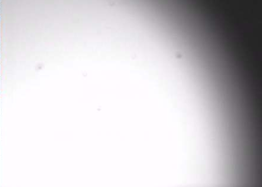
\includegraphics[width=0.7\linewidth]{before}
\caption{초점을 맞추기 전의 태양 표면}
\label{fig:before}
\end{figure}

\begin{figure}
\centering
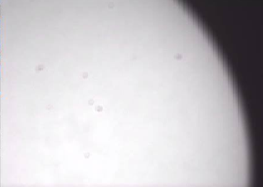
\includegraphics[width=0.7\linewidth]{after}
\caption{초점을 맞춘 후의 태양 표면}
\label{fig:after}
\end{figure}

\subsection{이론적 배경}

그림 3이 바로 Micro touch로, 시중에 나와있는 모터포커서이다. 이를 옆의 컴퓨터와 연결시킨 그림이 바로 그림4로, 이를 이용하여 컴퓨터에서도 ASCOM이라는 프로그램을 이용하여 원격으로 모터의 초점을 맞출 수 있도록 설정할 수가 있다. 그림3에서 나온 위의 두 버튼(IN, OUT)은 각각 초점을 맞추기 위해 망원경의 길이를 줄이거나 늘일 수 있는 버튼이다. Micro touch를 수동 혹은 자동으로 작동시켜 IN또는 OUT의 명령을 내렸을 경우, 그림 5에 보이는 모터포커서가 작동하게 된다. 이 모터포커서는 그림 5의 오른쪽에 보이는 모터를 움직여 천체망원경의 경통의 길이를 조절할 수 있도록 한다. 경통의 길이가 변화하면 그에 따라서 빛이 퍼지는 정도가 달라지므로 이를 잘 조정하면 망원경으로 관측하는 천체의 초점을 맞출 수 있게 된다.
\begin{figure}
\centering
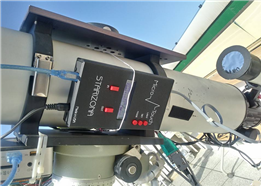
\includegraphics[width=0.7\linewidth]{telescope1}
\caption{Micro Touch를 천체망원경에 부착시킨 모습}
\label{fig:telescope1}
\end{figure}

\begin{figure}
\centering
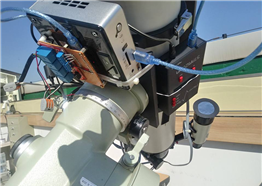
\includegraphics[width=0.7\linewidth]{telescope2}
\caption{Micro Touch와 연결된 컴퓨터}
\label{fig:telescope2}
\end{figure}

\begin{figure}
\centering
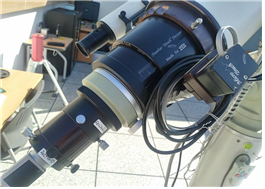
\includegraphics[width=0.7\linewidth]{telescope3}
\caption{모터포커서와 망원경의 길이}
\label{fig:telescope3}
\end{figure}

\subsection{선행연구 고찰}
이덕규 외(2014)는 복합재 광구조체와 결합하여 전자광학카메라의 영상품질을 향상시킬 수 있는 초점조절장치를 개발하였다.\cite{leedukgu2014}
\section{연구내용 및 방법}

\subsection{아두이노를 이용한 모터 포커서 제작}

모터 포커서 제작을 위하여 우리가 사용하는 것은 아두이노로, 기본적으로 모터의 구동을 위하여 아두이노를 이용하여 모터를 제어하는 펌웨어를 짜고 프로그램을 만든다. 이후 아두이노를 이용하여 모터를 돌릴 수 있게 해주는 회로를 짜서 직접 모터를 돌리는 작업을 한다.

\subsection{모터 포커서 구동 펌웨어 개발}

모터 포커서를 사용하기 위해서는 우리가 원하는 만큼 모터를 돌리는 것이 중요한데, 이를 아두이노로 구현하는 것이 필요하다. 직접 코딩을 하여 모커가 돌아가는 각도를 제어하는 것이 가능하게 하고, 이를 직접 모터 포커서에도 연결하여 작동을 제대로 하는지 확인한다. 또한 망원경에도 여러 가지 종류가 있기 때문에 직접 설정할 수 있는 설정창도 만들고, 버튼을 통하여 돌릴 수 있는 시스템을 구현한다. 또한, 통신을 위한 블루투스 통신 시스템과 망원경은 미세한 날씨변화에도 민감하므로 온습도 센서 또한 추가한다.

\subsection{모터 포커서 ASCOM 드라이버 개발 및 컴퓨터와의 연동}

모터 포커서를 활용하기 위해서는 별의 크기를 분석해서 돌려야 하므로 컴퓨터와의 연동이 필요하다. 따라서 모터 포커서의 ASCOM 드라이버를 제작해야 한다. ASCOM 드라이버를 이용하면 카메라로부터 정보를 컴퓨터가 받아서 데이터를 분석하고, 이 분석한 데이터를 이용하여 아두이노가 어떻게 조절해야 할지 명령을 내리면 ASCOM 드라이버를 통해 정보를 전달하여 모터가 제어한 대로 조절할 수 있도록 구현한다.

\subsection{카메라(또는 CCD) 제어 프로그램 개발}

사진 관측을 이용해서 얻은 사진을 컴퓨터로 연결하여 분석할 수 있도록 해야 한다. 그러기 위해서는 사진을 컴퓨터로 보낼 수 있어야 한다. 또한, 카메라에 나오는 화면의 변화를 보아야 하므로 연속적인 변화를 보낼 수 있는 프로그램을 만들어서 컴퓨터가 제대로 인식을 할 수 있는지 확인한다.

\subsection{오토 포커싱 알고리즘 개발 및 구현}

천체망원경의 초점을 맞추기 위해 사진 관측의 사진을 연속적으로 찍어서 컴퓨터로 보내주고, 컴퓨터는 이를 분석하여 모터 포커서 컨트롤러에 별의 크기가 커지고 있는지 작아지고 있는지 정보를 알고리즘에 보내준다. 그러면 프로그래밍 된 아두이노가 모터를 어느 방향으로 돌려야 하는지 판단하여 모터를 돌리고, 이 과정을 반복하여 별의 크기가 제일 작아질 때, 즉 별의 초점이 맞을 때 이 과정을 멈춘다.

\section{연구결과의 활용과 기대효과}

이전 제품인 Micro Touch 제품을 사용하다가 든 생각은 일단 가속기능이 없어서 높은 수치로 올려야 할때 시간이 조금 걸려서 불편하다는 생각을 하였고, 길이당 모터가 돌아가는 각도를 표시해 주지 않아서 불편한 것도 있었다. 우리가 구현한 모터 드라이버는 이러한 기능이 추가되어 있어 직접 사용하다가 느낀 불편한 점을 없앰으로서 사용하는 사람들에게 편리함을 제공할 수 있다. 또한, Micro Touch의 경우에는 가격이 매우 비쌌는데, 아두이노로 구현을 한다면 훨씬 저렴한 가격에 이러한 시스템을 구동하는 것이 가능해 질 것이다. 이렇게 구현한 자동초점조절 모터포커싱 시스템이 상용화 된다면 사람들은 더욱 싼 가격에 이러한 기능을 얻을 수 있을 것이고, 또한 원래의 장점과 같이 천체를 관측하거나 연구활동에 천체 망원경에서 초점을 맞춰야 하는 일이 생겼을 때 사람의 손보다 훨씬 빠르고 정확하게 초점을 맞추는 것이 가능해질 것이다.

\bibliography{bibfile} % 참고문헌

\end{document}